\chapter{Module CAN et g�n�ricit�}
\authors{
  \authorinfo{Julien}{Peeters} \\
  \authorinfo{Fabien}{Provost} \\
  \authorinfo{Feng}{Xiong} \\
  \authorinfo{Yongchao}{Xu}
  
}

\section{I2C Slave}


\begin{figure}[htpb]
  \centering
  \fbox{
    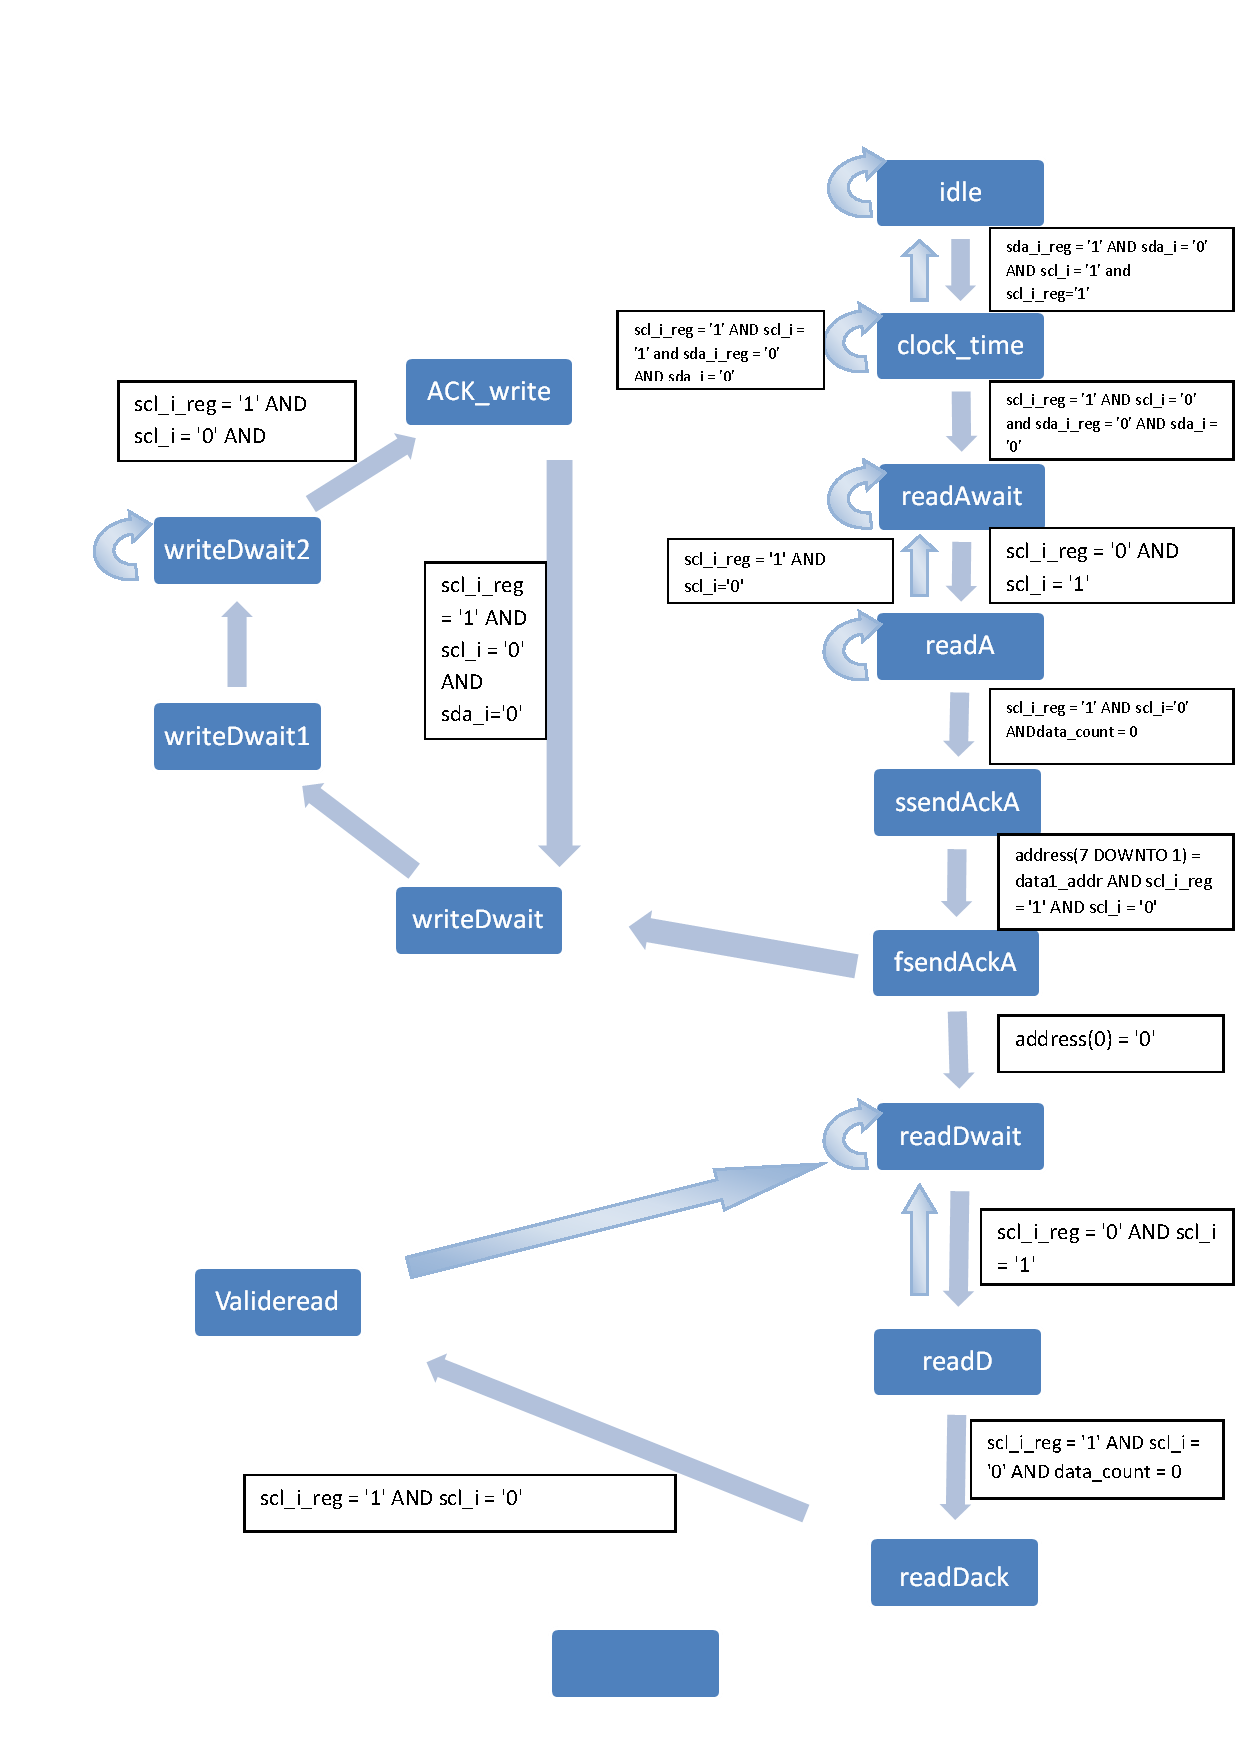
\includegraphics[scale=0.9]{images/diagramme_slave_i2c}
  }
  \caption{Automate de PCF}
  \label{fig:Automate_PCF}
\end{figure}

\section{Description et contexte}
L'objecif de cette partie est de cr�er des outils permettant de simplifier l'utilisation des diff�rents bus de mani�re g�n�rique de fa�on � pouvoir �tre r�utilis� � plusieurs endroits du projet.

Seront vu dans cette partie, la conception et le d�veloppement des noeuds CAN qui permettent de recevoir 
des messages CAN et de les interpr�ter afin de g�n�rer les actions ad�quates (envoie de messages I$^2$C par 
exemple) et inversement (envoie de message CAN apr�s utilisation d'un actionneur), aussi nous verrons
l'utilisation d'un FPGA comme interface au bus I$^2$C, c'est � dire que le bloc qui permet de connecter 
des DEL, des boutons poussoirs ou autre composants plus complexes � un bus I$^2$C. 

\section{Noeud CAN/I$^2$C}
\subsection{Objectifs}
L'objectif de ce module est donc double
\begin{itemize}
\item la recherche de modifications sur le bus I$^2$C, puis envoie des changements par messages CAN
\item traiter les messages CAN re�us et envoie de messages I$^2$C aux esclaves concern�s 

\end{itemize}
